\documentclass[twoside]{book}

% Packages required by doxygen
\usepackage{fixltx2e}
\usepackage{calc}
\usepackage{doxygen}
\usepackage[export]{adjustbox} % also loads graphicx
\usepackage{graphicx}
\usepackage[utf8]{inputenc}
\usepackage{makeidx}
\usepackage{multicol}
\usepackage{multirow}
\PassOptionsToPackage{warn}{textcomp}
\usepackage{textcomp}
\usepackage[nointegrals]{wasysym}
\usepackage[table]{xcolor}

% Font selection
\usepackage[T1]{fontenc}
\usepackage[scaled=.90]{helvet}
\usepackage{courier}
\usepackage{amssymb}
\usepackage{sectsty}
\renewcommand{\familydefault}{\sfdefault}
\allsectionsfont{%
  \fontseries{bc}\selectfont%
  \color{darkgray}%
}
\renewcommand{\DoxyLabelFont}{%
  \fontseries{bc}\selectfont%
  \color{darkgray}%
}
\newcommand{\+}{\discretionary{\mbox{\scriptsize$\hookleftarrow$}}{}{}}

% Page & text layout
\usepackage{geometry}
\geometry{%
  a4paper,%
  top=2.5cm,%
  bottom=2.5cm,%
  left=2.5cm,%
  right=2.5cm%
}
\tolerance=750
\hfuzz=15pt
\hbadness=750
\setlength{\emergencystretch}{15pt}
\setlength{\parindent}{0cm}
\setlength{\parskip}{3ex plus 2ex minus 2ex}
\makeatletter
\renewcommand{\paragraph}{%
  \@startsection{paragraph}{4}{0ex}{-1.0ex}{1.0ex}{%
    \normalfont\normalsize\bfseries\SS@parafont%
  }%
}
\renewcommand{\subparagraph}{%
  \@startsection{subparagraph}{5}{0ex}{-1.0ex}{1.0ex}{%
    \normalfont\normalsize\bfseries\SS@subparafont%
  }%
}
\makeatother

% Headers & footers
\usepackage{fancyhdr}
\pagestyle{fancyplain}
\fancyhead[LE]{\fancyplain{}{\bfseries\thepage}}
\fancyhead[CE]{\fancyplain{}{}}
\fancyhead[RE]{\fancyplain{}{\bfseries\leftmark}}
\fancyhead[LO]{\fancyplain{}{\bfseries\rightmark}}
\fancyhead[CO]{\fancyplain{}{}}
\fancyhead[RO]{\fancyplain{}{\bfseries\thepage}}
\fancyfoot[LE]{\fancyplain{}{}}
\fancyfoot[CE]{\fancyplain{}{}}
\fancyfoot[RE]{\fancyplain{}{\bfseries\scriptsize Generated by Doxygen }}
\fancyfoot[LO]{\fancyplain{}{\bfseries\scriptsize Generated by Doxygen }}
\fancyfoot[CO]{\fancyplain{}{}}
\fancyfoot[RO]{\fancyplain{}{}}
\renewcommand{\footrulewidth}{0.4pt}
\renewcommand{\chaptermark}[1]{%
  \markboth{#1}{}%
}
\renewcommand{\sectionmark}[1]{%
  \markright{\thesection\ #1}%
}

% Indices & bibliography
\usepackage{natbib}
\usepackage[titles]{tocloft}
\setcounter{tocdepth}{3}
\setcounter{secnumdepth}{5}
\makeindex

% Hyperlinks (required, but should be loaded last)
\usepackage{ifpdf}
\ifpdf
  \usepackage[pdftex,pagebackref=true]{hyperref}
\else
  \usepackage[ps2pdf,pagebackref=true]{hyperref}
\fi
\hypersetup{%
  colorlinks=true,%
  linkcolor=blue,%
  citecolor=blue,%
  unicode%
}

% Custom commands
\newcommand{\clearemptydoublepage}{%
  \newpage{\pagestyle{empty}\cleardoublepage}%
}

\usepackage{caption}
\captionsetup{labelsep=space,justification=centering,font={bf},singlelinecheck=off,skip=4pt,position=top}

%===== C O N T E N T S =====

\begin{document}

% Titlepage & ToC
\hypersetup{pageanchor=false,
             bookmarksnumbered=true,
             pdfencoding=unicode
            }
\pagenumbering{alph}
\begin{titlepage}
\vspace*{7cm}
\begin{center}%
{\Large Dice Roler }\\
\vspace*{1cm}
{\large Generated by Doxygen 1.8.13}\\
\end{center}
\end{titlepage}
\clearemptydoublepage
\pagenumbering{roman}
\tableofcontents
\clearemptydoublepage
\pagenumbering{arabic}
\hypersetup{pageanchor=true}

%--- Begin generated contents ---
\chapter{File Index}
\section{File List}
Here is a list of all documented files with brief descriptions\+:\begin{DoxyCompactList}
\item\contentsline{section}{/home/marques/\+Desktop/\+Cesium/\+D\+P\+U\+M/2\+\_\+reverse\+\_\+staircase/code\+\_\+golf/\+Marquinhos87/\+C/src/\hyperlink{stair_8h}{stair.\+h} }{\pageref{stair_8h}}{}
\end{DoxyCompactList}

\chapter{File Documentation}
\hypertarget{diceroler_8h}{}\section{/home/marques/\+Desktop/\+Cesium/\+D\+P\+U\+M/1\+\_\+dice\+\_\+roler/code\+\_\+golf/\+Marquinhos87/\+C/src/diceroler.h File Reference}
\label{diceroler_8h}\index{/home/marques/\+Desktop/\+Cesium/\+D\+P\+U\+M/1\+\_\+dice\+\_\+roler/code\+\_\+golf/\+Marquinhos87/\+C/src/diceroler.\+h@{/home/marques/\+Desktop/\+Cesium/\+D\+P\+U\+M/1\+\_\+dice\+\_\+roler/code\+\_\+golf/\+Marquinhos87/\+C/src/diceroler.\+h}}
{\ttfamily \#include $<$stdio.\+h$>$}\newline
{\ttfamily \#include $<$stdlib.\+h$>$}\newline
{\ttfamily \#include $<$string.\+h$>$}\newline
{\ttfamily \#include $<$time.\+h$>$}\newline
{\ttfamily \#include $<$ctype.\+h$>$}\newline
Include dependency graph for diceroler.\+h\+:\nopagebreak
\begin{figure}[H]
\begin{center}
\leavevmode
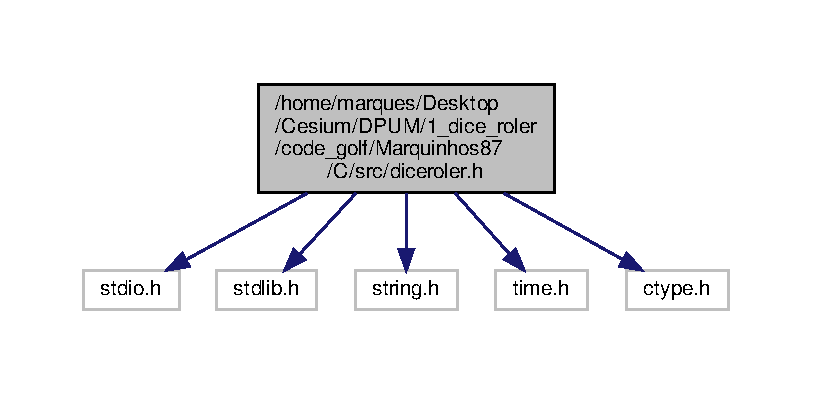
\includegraphics[width=350pt]{diceroler_8h__incl}
\end{center}
\end{figure}
\subsection*{Functions}
\begin{DoxyCompactItemize}
\item 
int \hyperlink{diceroler_8h_a4e9c274287e91e69632a10c25aa19c44}{getD} (char $\ast$l)
\item 
int \hyperlink{diceroler_8h_a7800ab7b7564ba44ff219de7f3d19f32}{getF} (char $\ast$l)
\item 
int $\ast$ \hyperlink{diceroler_8h_a8ae17648d8acdac6e1beea61c0ae9fea}{genV} (int d, int f)
\item 
void \hyperlink{diceroler_8h_a784c2f0f86fdcaf4f18a53f33ec36c76}{prt} (int d, int v, int $\ast$vs)
\item 
int \hyperlink{diceroler_8h_ad39671e47ead404e4e9ad0257ad57f72}{sum} (int d, int $\ast$v)
\item 
int \hyperlink{diceroler_8h_ab25ea6343d892b5e77002d6227a69e28}{calc} (char $\ast$l)
\end{DoxyCompactItemize}
\subsection*{Variables}
\begin{DoxyCompactItemize}
\item 
int \hyperlink{diceroler_8h_a6150e0515f7202e2fb518f7206ed97dc}{x}
\end{DoxyCompactItemize}


\subsection{Function Documentation}
\mbox{\Hypertarget{diceroler_8h_ab25ea6343d892b5e77002d6227a69e28}\label{diceroler_8h_ab25ea6343d892b5e77002d6227a69e28}} 
\index{diceroler.\+h@{diceroler.\+h}!calc@{calc}}
\index{calc@{calc}!diceroler.\+h@{diceroler.\+h}}
\subsubsection{\texorpdfstring{calc()}{calc()}}
{\footnotesize\ttfamily int calc (\begin{DoxyParamCaption}\item[{char $\ast$}]{l }\end{DoxyParamCaption})}

Function that calls the others to generate de final result


\begin{DoxyParams}{Parameters}
{\em l} & String to process. \\
\hline
\end{DoxyParams}
\begin{DoxyReturn}{Returns}
Return 0 if alright OK or 1 if something wrong 
\end{DoxyReturn}
\mbox{\Hypertarget{diceroler_8h_a8ae17648d8acdac6e1beea61c0ae9fea}\label{diceroler_8h_a8ae17648d8acdac6e1beea61c0ae9fea}} 
\index{diceroler.\+h@{diceroler.\+h}!genV@{genV}}
\index{genV@{genV}!diceroler.\+h@{diceroler.\+h}}
\subsubsection{\texorpdfstring{gen\+V()}{genV()}}
{\footnotesize\ttfamily int$\ast$ genV (\begin{DoxyParamCaption}\item[{int}]{d,  }\item[{int}]{f }\end{DoxyParamCaption})}

Funtion that generate numbers between \textquotesingle{}1 to f\textquotesingle{} in a total of \textquotesingle{}d\textquotesingle{} times.


\begin{DoxyParams}{Parameters}
{\em d} & Number of dices. \\
\hline
{\em f} & Number of faces. \\
\hline
\end{DoxyParams}
\begin{DoxyReturn}{Returns}
The Integer array with de values of the all dices 
\end{DoxyReturn}
\mbox{\Hypertarget{diceroler_8h_a4e9c274287e91e69632a10c25aa19c44}\label{diceroler_8h_a4e9c274287e91e69632a10c25aa19c44}} 
\index{diceroler.\+h@{diceroler.\+h}!getD@{getD}}
\index{getD@{getD}!diceroler.\+h@{diceroler.\+h}}
\subsubsection{\texorpdfstring{get\+D()}{getD()}}
{\footnotesize\ttfamily int getD (\begin{DoxyParamCaption}\item[{char $\ast$}]{l }\end{DoxyParamCaption})}

Function that parse the string to get the number of dices.


\begin{DoxyParams}{Parameters}
{\em l} & a charater pointer. \\
\hline
\end{DoxyParams}
\begin{DoxyReturn}{Returns}
The number of dices 
\end{DoxyReturn}
\mbox{\Hypertarget{diceroler_8h_a7800ab7b7564ba44ff219de7f3d19f32}\label{diceroler_8h_a7800ab7b7564ba44ff219de7f3d19f32}} 
\index{diceroler.\+h@{diceroler.\+h}!getF@{getF}}
\index{getF@{getF}!diceroler.\+h@{diceroler.\+h}}
\subsubsection{\texorpdfstring{get\+F()}{getF()}}
{\footnotesize\ttfamily int getF (\begin{DoxyParamCaption}\item[{char $\ast$}]{l }\end{DoxyParamCaption})}

Function that parse the string to get the number of faces of the dices.


\begin{DoxyParams}{Parameters}
{\em l} & a charater pointer. \\
\hline
\end{DoxyParams}
\begin{DoxyReturn}{Returns}
The number of faces of every dice 
\end{DoxyReturn}
\mbox{\Hypertarget{diceroler_8h_a784c2f0f86fdcaf4f18a53f33ec36c76}\label{diceroler_8h_a784c2f0f86fdcaf4f18a53f33ec36c76}} 
\index{diceroler.\+h@{diceroler.\+h}!prt@{prt}}
\index{prt@{prt}!diceroler.\+h@{diceroler.\+h}}
\subsubsection{\texorpdfstring{prt()}{prt()}}
{\footnotesize\ttfamily void prt (\begin{DoxyParamCaption}\item[{int}]{d,  }\item[{int}]{v,  }\item[{int $\ast$}]{vs }\end{DoxyParamCaption})}

Function to print to stdout the result of a play or multiple-\/play.


\begin{DoxyParams}{Parameters}
{\em d} & Number of dices. \\
\hline
{\em v} & Sum of the values of all dices. \\
\hline
{\em vs} & Integer array with all values of the dices. \\
\hline
\end{DoxyParams}
\mbox{\Hypertarget{diceroler_8h_ad39671e47ead404e4e9ad0257ad57f72}\label{diceroler_8h_ad39671e47ead404e4e9ad0257ad57f72}} 
\index{diceroler.\+h@{diceroler.\+h}!sum@{sum}}
\index{sum@{sum}!diceroler.\+h@{diceroler.\+h}}
\subsubsection{\texorpdfstring{sum()}{sum()}}
{\footnotesize\ttfamily int sum (\begin{DoxyParamCaption}\item[{int}]{d,  }\item[{int $\ast$}]{v }\end{DoxyParamCaption})}

Function that make de sum of all dices rolled.


\begin{DoxyParams}{Parameters}
{\em d} & Number of dices. \\
\hline
{\em v} & Integer array with all values of the dices. \\
\hline
\end{DoxyParams}
\begin{DoxyReturn}{Returns}
The sum of all dices rolled 
\end{DoxyReturn}


\subsection{Variable Documentation}
\mbox{\Hypertarget{diceroler_8h_a6150e0515f7202e2fb518f7206ed97dc}\label{diceroler_8h_a6150e0515f7202e2fb518f7206ed97dc}} 
\index{diceroler.\+h@{diceroler.\+h}!x@{x}}
\index{x@{x}!diceroler.\+h@{diceroler.\+h}}
\subsubsection{\texorpdfstring{x}{x}}
{\footnotesize\ttfamily int x}

This is a global variable to save the current position of the line that we are processing. 
%--- End generated contents ---

% Index
\backmatter
\newpage
\phantomsection
\clearemptydoublepage
\addcontentsline{toc}{chapter}{Index}
\printindex

\end{document}
